% parcours de graphes 

\begin{frame}{Parcours de graphe}
\begin{itemize}
    \item Comment parcourir un graphe de façon exhaustive ?
    \item Explorer tous les sommets 
    \begin{itemize}
        \item En partant d'un sommet d'origine (ou plusieurs si le graphe n'est pas connexe / fortement connexe)
        \item En suivant uniquement les arcs qui sortent d'un sommet déjà exploré
        \item En construisant un historique de son parcours : notion d'arbre de \emph{parcours}
    \end{itemize}
    \item Routine de base en algorithmique des graphes 
\end{itemize}
\end{frame}

\begin{frame}{Comment ?}
    \begin{center}
        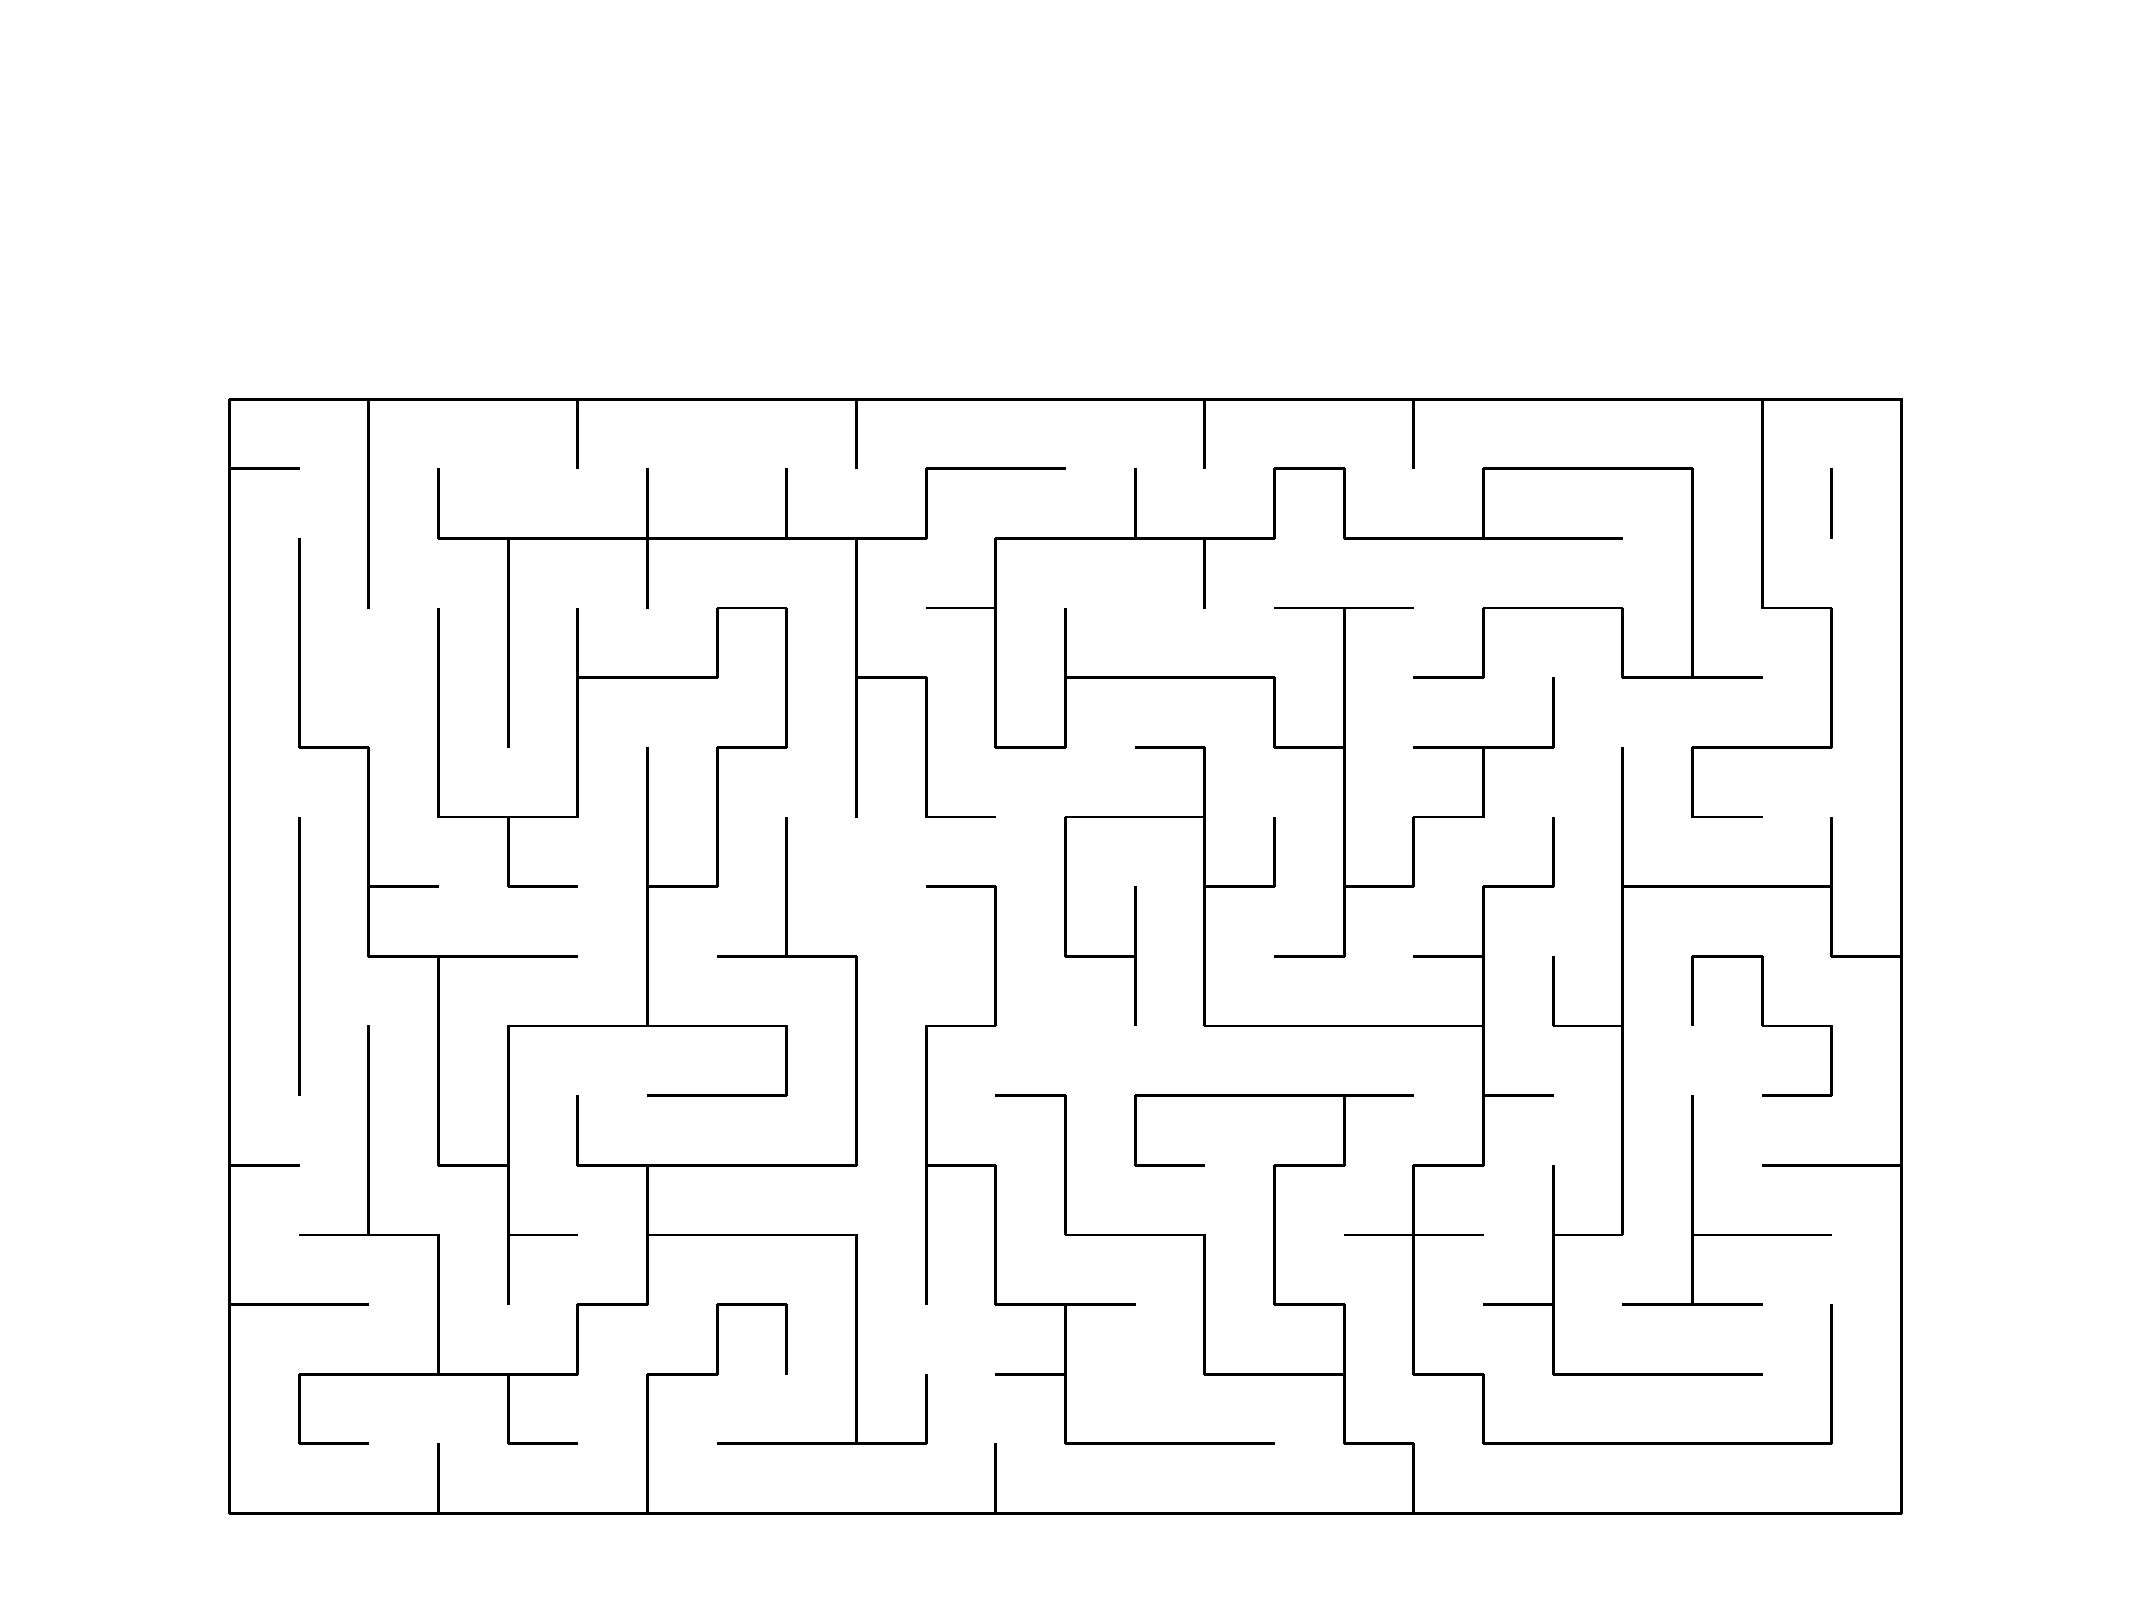
\includegraphics[width=.75\textwidth]{fig/labyrinthe.pdf}
    \end{center}
\end{frame}

\begin{frame}{Comment ?}
    \begin{center}
        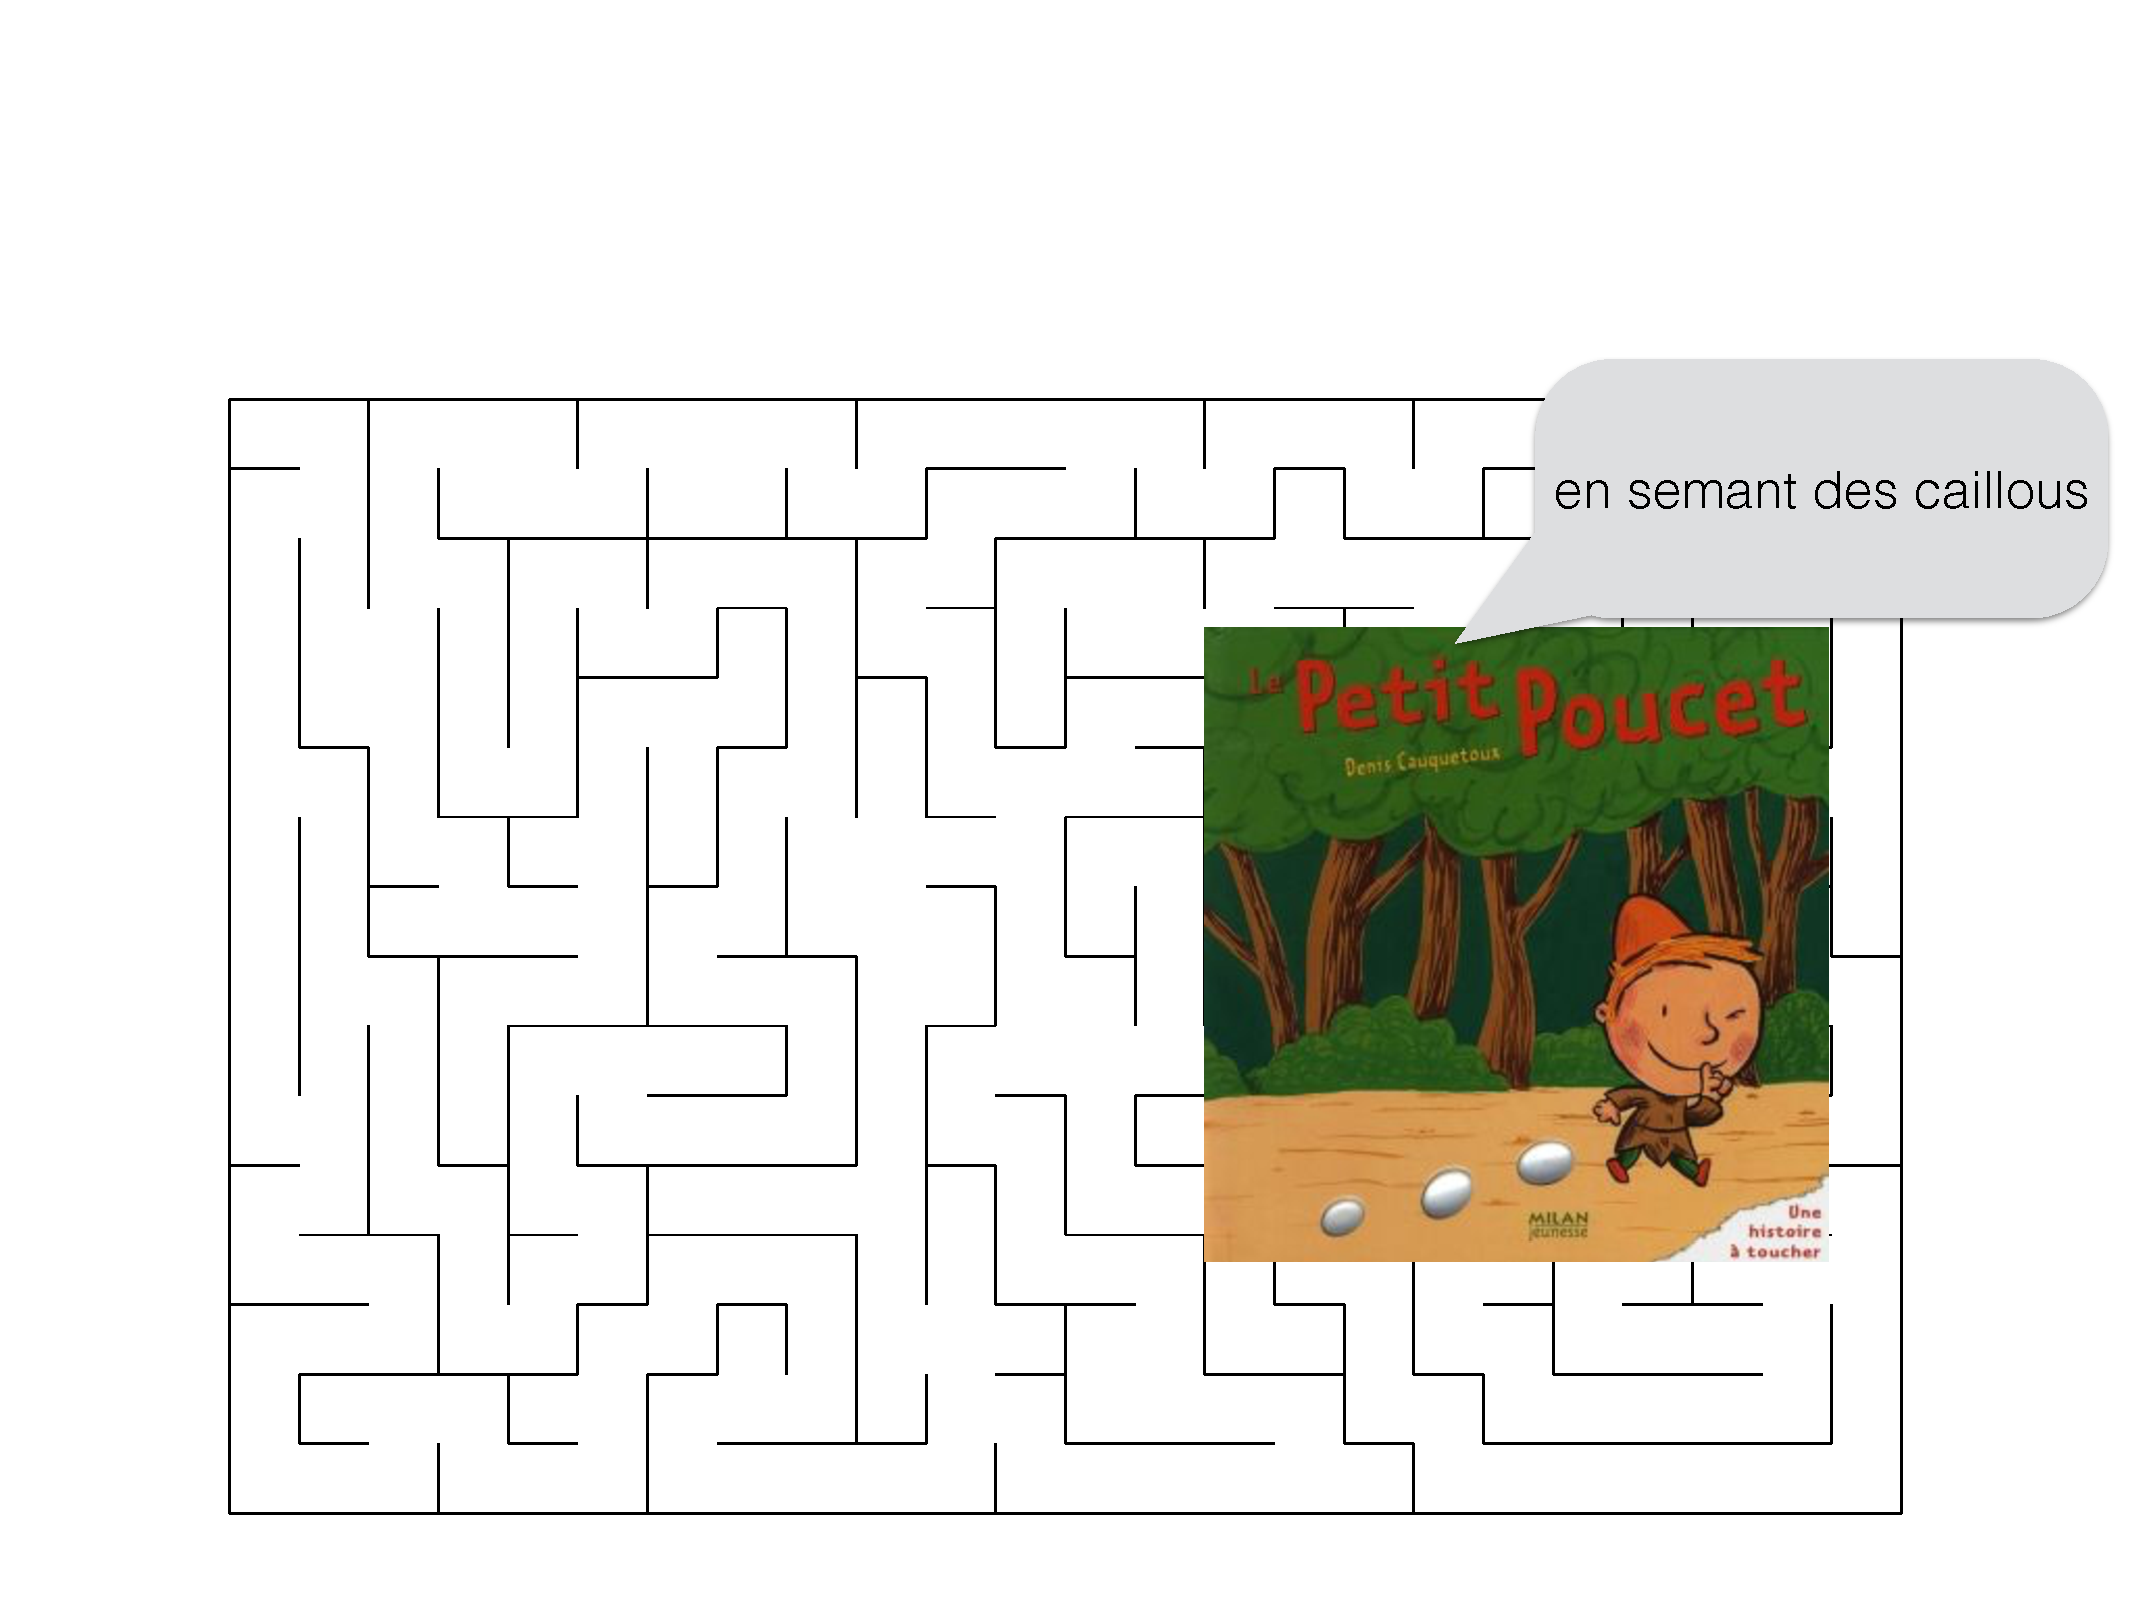
\includegraphics[width=.75\textwidth]{fig/labyrinthe-cailloux.pdf}
    \end{center}
\end{frame}

\begin{frame}{Comment ?}
    \begin{center}
        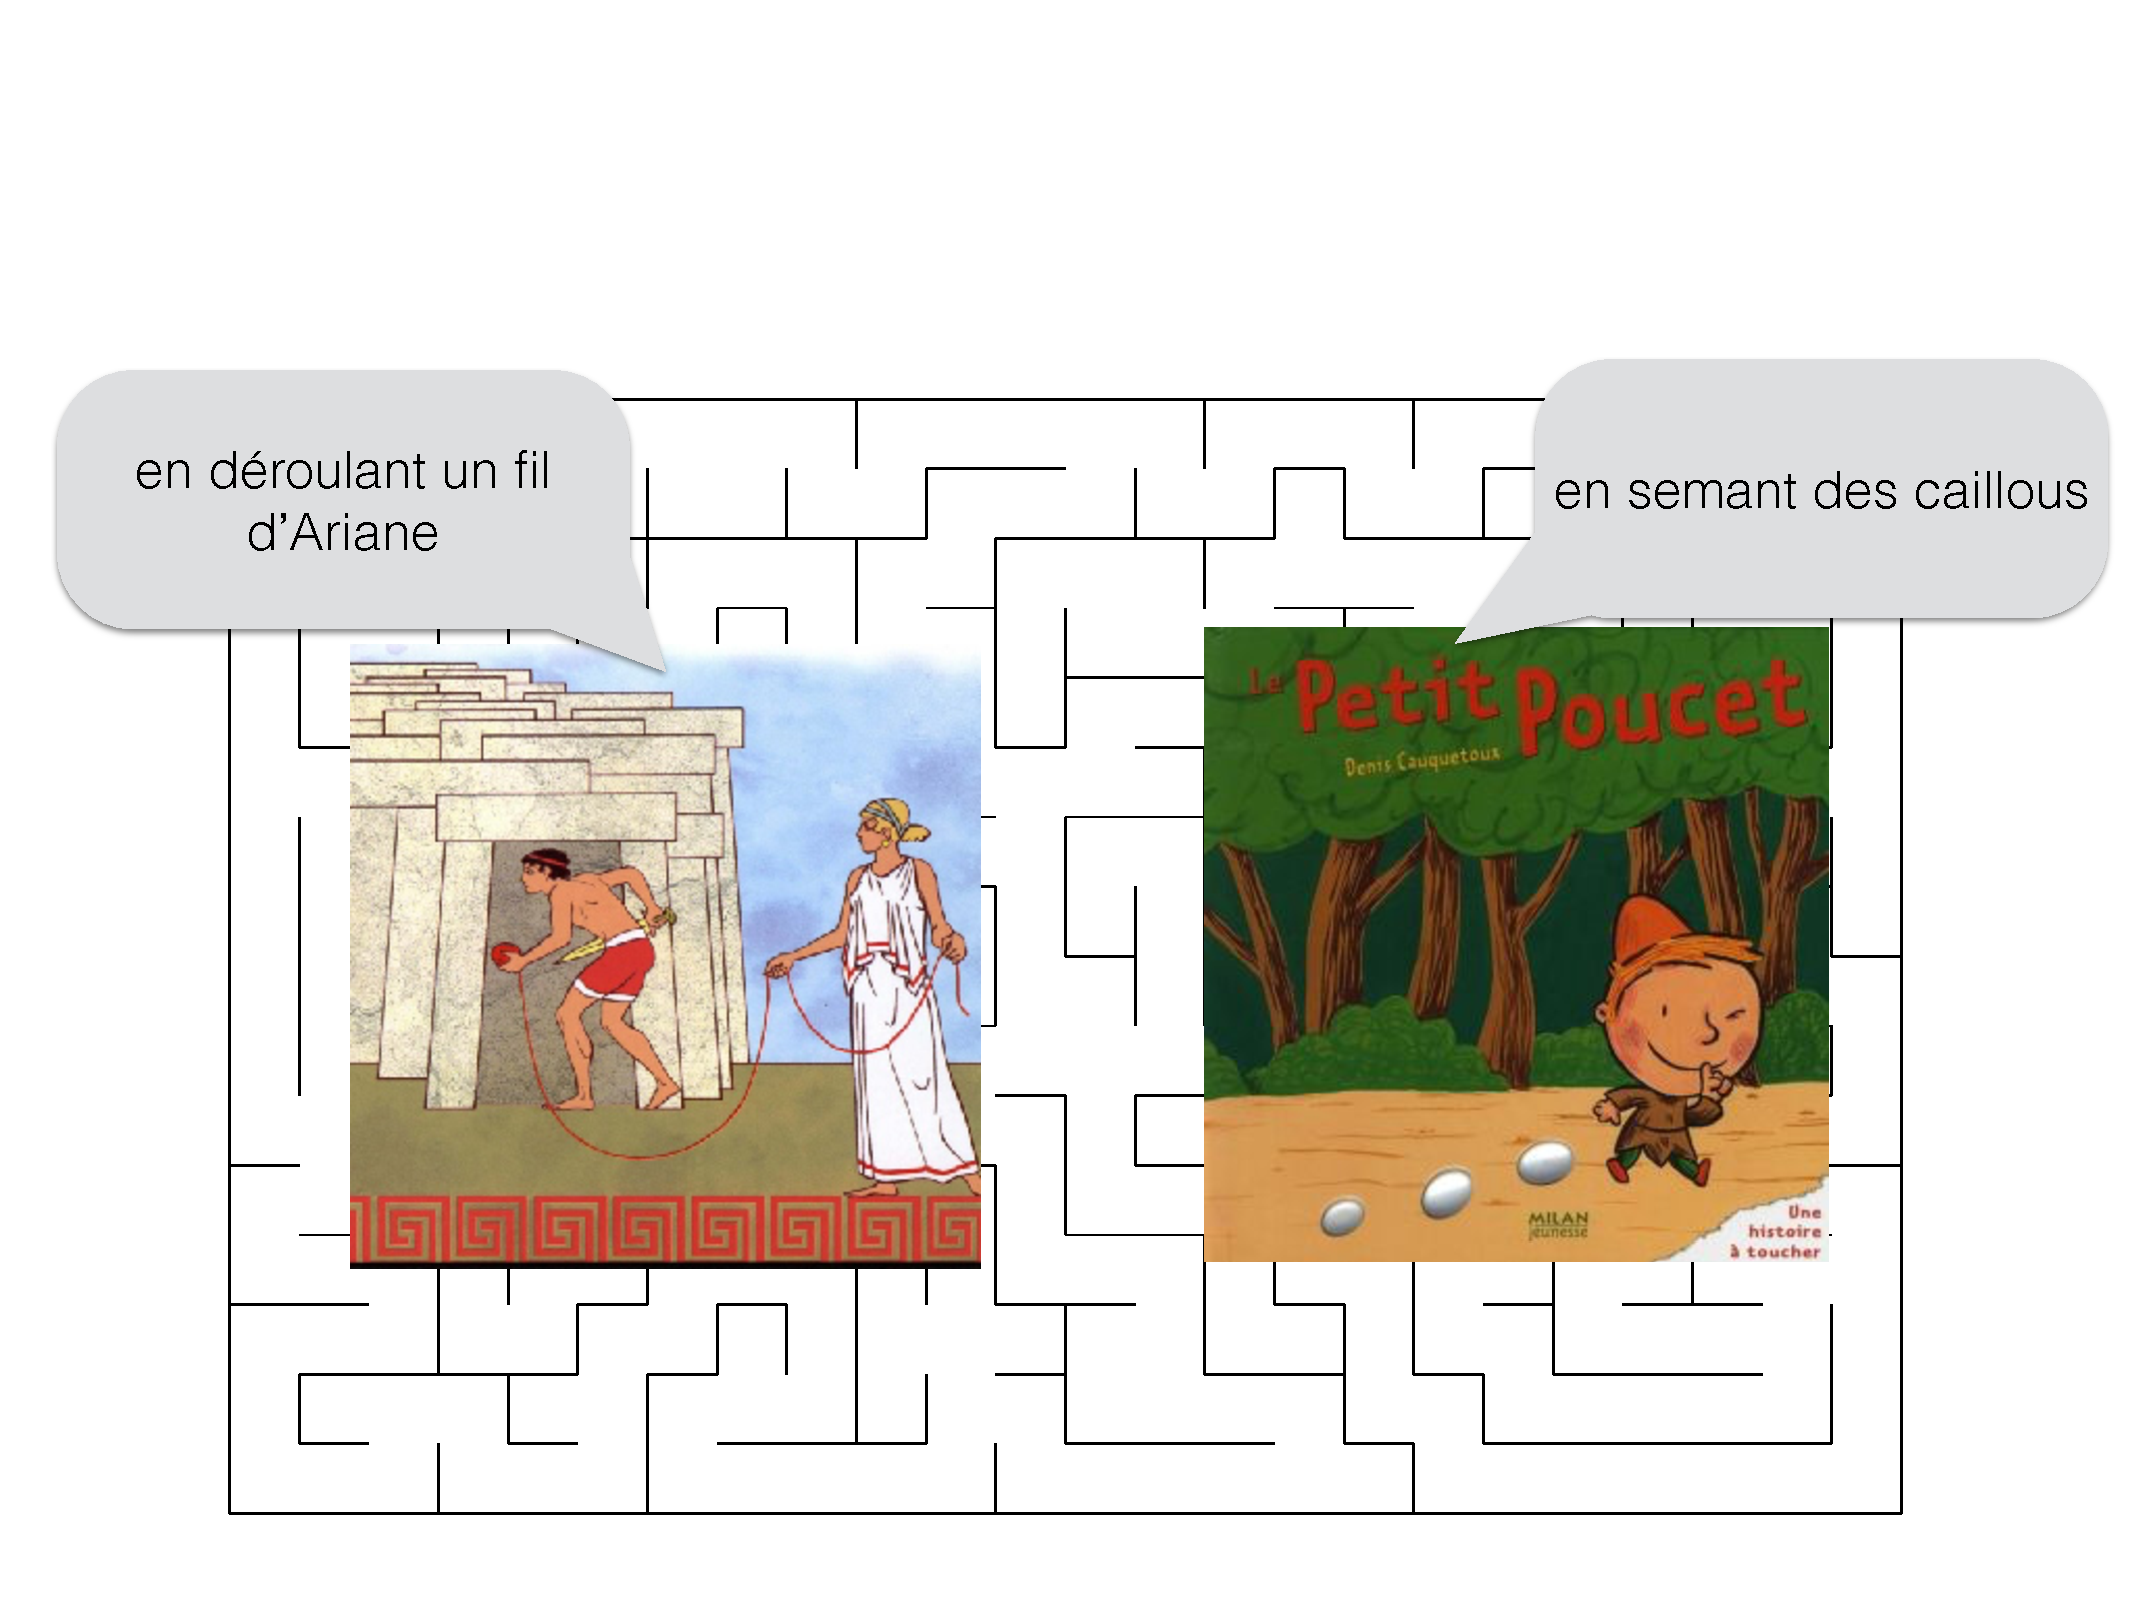
\includegraphics[width=.75\textwidth]{fig/labyrinthe-3.pdf}
    \end{center}
\end{frame}

\begin{frame}[fragile]
\frametitle{Parcours en profondeur}
    \begin{itemize}
        \item On utilise un tableau de booléens 
        \begin{itemize}
            \item \emph{vrai} si le sommet a été vu 
            \item \emph{faux} sinon 
        \end{itemize}
        \item on construit une fonction récursive \texttt{visite(i)} qui va explorer les sommets non vus à partir de $i$ ($i$ inclus)
    \end{itemize}
    
    % test
    \begin{algorithm}[H]
        \begin{algorithmic}[1]
            \Function{visite}{$i$ : sommet}
            \State vu[i] \gets true
            \For{$j \in Adj[i]$}
                \If{$vu[j] = false$}
                    \State visite(j)
                \EndIf
            \EndFor
            \EndFunction
         \end{algorithmic}
        \caption{Parcours en profondeur à partir d'un sommet}
        \label{alg:prof:visite}
        \end{algorithm}
\end{frame}



% ajouter la version avec les dates de visite ? pas sûr de l'intérêt ici...

\begin{frame}{Parcours en profondeur}
    \begin{itemize}
        \item Attention : l'algorithme n'est pas correct pour parcourir tout le graphe
        \item De fait, il ne fonctionne que si le graphe est connexe 
        \pause 
        \item On peut ajouter une boucle sur tous les sommets 
        \pause 
        \begin{algorithm}[H]
            \begin{algorithmic}[1]
                \State vu \gets [$false$,...,$false$]
                \For{$i \in S$}
                    \If{$vu[i] = false$}
                        \State visite(i)
                    \EndIf
                \EndFor
             \end{algorithmic}
            \caption{Parcours en profondeur}
            \label{alg:prof:alg}
            \end{algorithm}
        \pause 
        \item convention implicite : on parcourt les sommets et les adjacents en ordre croissant
    \end{itemize}
\end{frame}


\directlua{\detokenize{
    for i=0,6,1 do
        tex.sprint("\\begin{frame}{Exemple} \\input{genfig/pp-", i, ".tex} \\end{frame}")
    end
}}

\begin{frame}{Efficacité de l'algorithme}
    \begin{itemize}
        \item On marque $vu[i]$ une seule fois 
        \begin{itemize}
            \item Donc \texttt{visite(i)} termine toujours
            \item \texttt{visite(i)} n'est appelée qu'une seule fois par sommet
        \end{itemize}
        \item Le temps de calcul est dominé par les itérations de boucles
        \begin{itemize}
            \item La boucle principale s'exécute $n$ fois 
            \item La boucle secondaire s'exécute globalement $\sum_i | Adj[i] | = m$
        \end{itemize}
        \item La complexité pire cas est en $n+m$, donc linéaire
    \end{itemize}
\end{frame}

\begin{frame}{Forêts de parcours}
    \begin{itemize}
        \item Pendant un parcours en profondeur récursif, on peut créer une relation \emph{parent} qui mémorise pour chaque sommet $j$ 
        \begin{itemize}
            \item le sommet $i$ responsable de sa visite 
            \item $-1$ si le sommet $j$ est visité par la boucle principale 
        \end{itemize}
        \item Le graphe non-orienté associé à \emph{parent} (une arête entre $i$ et $j$ si $parent[i]=j$), forme une forêt de parcours 
    \end{itemize}
\end{frame}



\begin{frame}[fragile]
\frametitle{Algorithme}
    \begin{columns}
        \begin{column}{.5\textwidth}
            \begin{algorithmic}[1]
                \Function{visite}{$i$ : sommet}
                \State vu[i] \gets true
                \For{$j \in Adj[i]$}
                    \If{$vu[j] = false$}
                        \State \textcolor{blue}{parent[j] \gets i}
                        \State visite(j)
                    \EndIf
                \EndFor
                \EndFunction
            \end{algorithmic}
        \end{column}
        \begin{column}{.5\textwidth}
            \begin{algorithmic}[1]
                \State vu \gets [$false$,...,$false$]
                \State \textcolor{blue}{parent \gets [$-1$,...,$-1$]}
                \For{$i \in S$}
                    \If{$vu[i] = false$}
                    \State visite(i)
                    \EndIf
                \EndFor
                \end{algorithmic}            
        \end{column}
    \end{columns}    
\end{frame}


% ajouter un exemple sur les forets de parcours 
% cours David : 
%  un exemple jouet que je ne comprends pas 
%  un exemple de parcours sur un très grand graphe 

\begin{frame}{Exemples d'application}
    \begin{itemize}
        \item Les arbres (forêts) de parcours ont diverses applications
        \item Composantes connexes 
        \begin{itemize}
            \item Identification
            \item Parcours 
        \end{itemize}
        \item Graphe bipartis
    \end{itemize}
\end{frame}


\begin{frame}{Composantes connexes}
    \begin{itemize}
        \item Propriétés du parcours en profondeur
        \begin{itemize}
            \item \texttt{visite(i)} ne parcourt que les sommets accessibles depuis $i$ 
            \item elle parcourt tous ceux qui n'étaient pas marqués \texttt{vu} avant de démarrer la fonction 
        \end{itemize}
        \item Comptage du nombre de composantes connexes 
        \begin{itemize}
            \item Il suffit de rajouter un compteur dans la boucle principale 
            \item incrémenté à chaque appel à \texttt{visite(i)}
        \end{itemize}
    \end{itemize}
    \begin{center}
        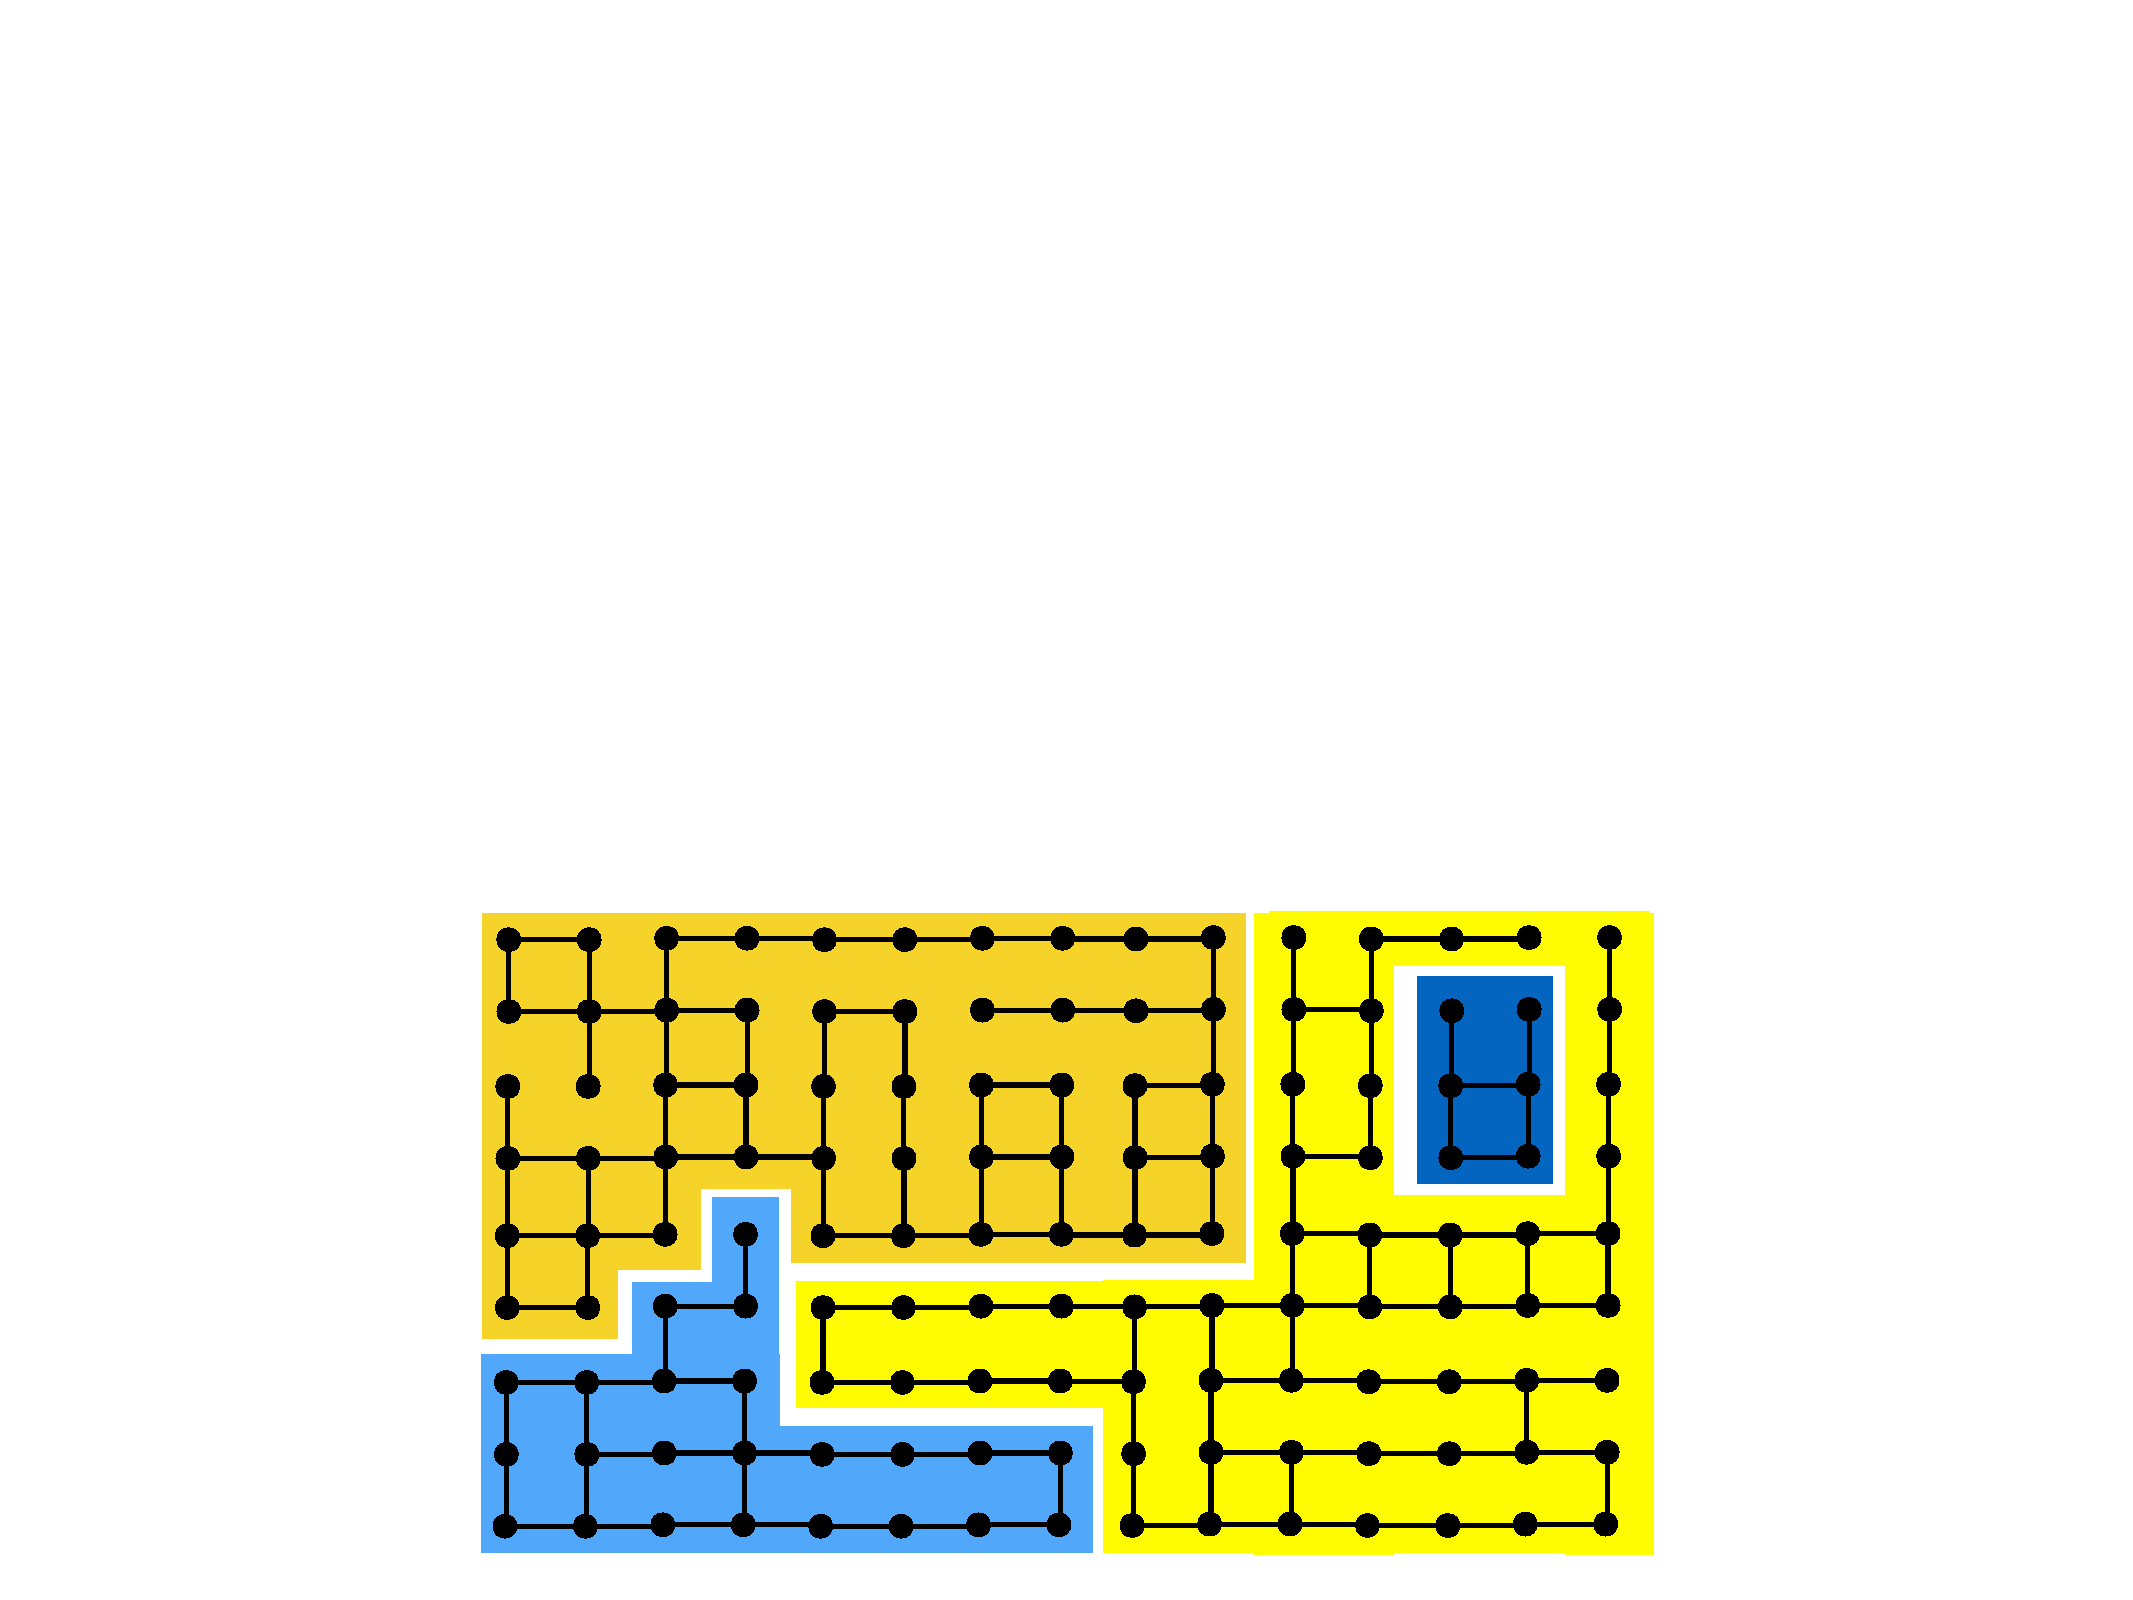
\includegraphics[width=.5\textwidth]{fig/cc.pdf}
    \end{center}
\end{frame}

\begin{frame}{Graphe biparti : plan de table}
    \begin{example}
        Pour un repas de famille, on doit réaliser un plan de table en tenant compte des inimitiés : les personnes qui ne s'aiment pas ne doivent pas se retrouver à la même table.        
    \end{example}
    \begin{center}
        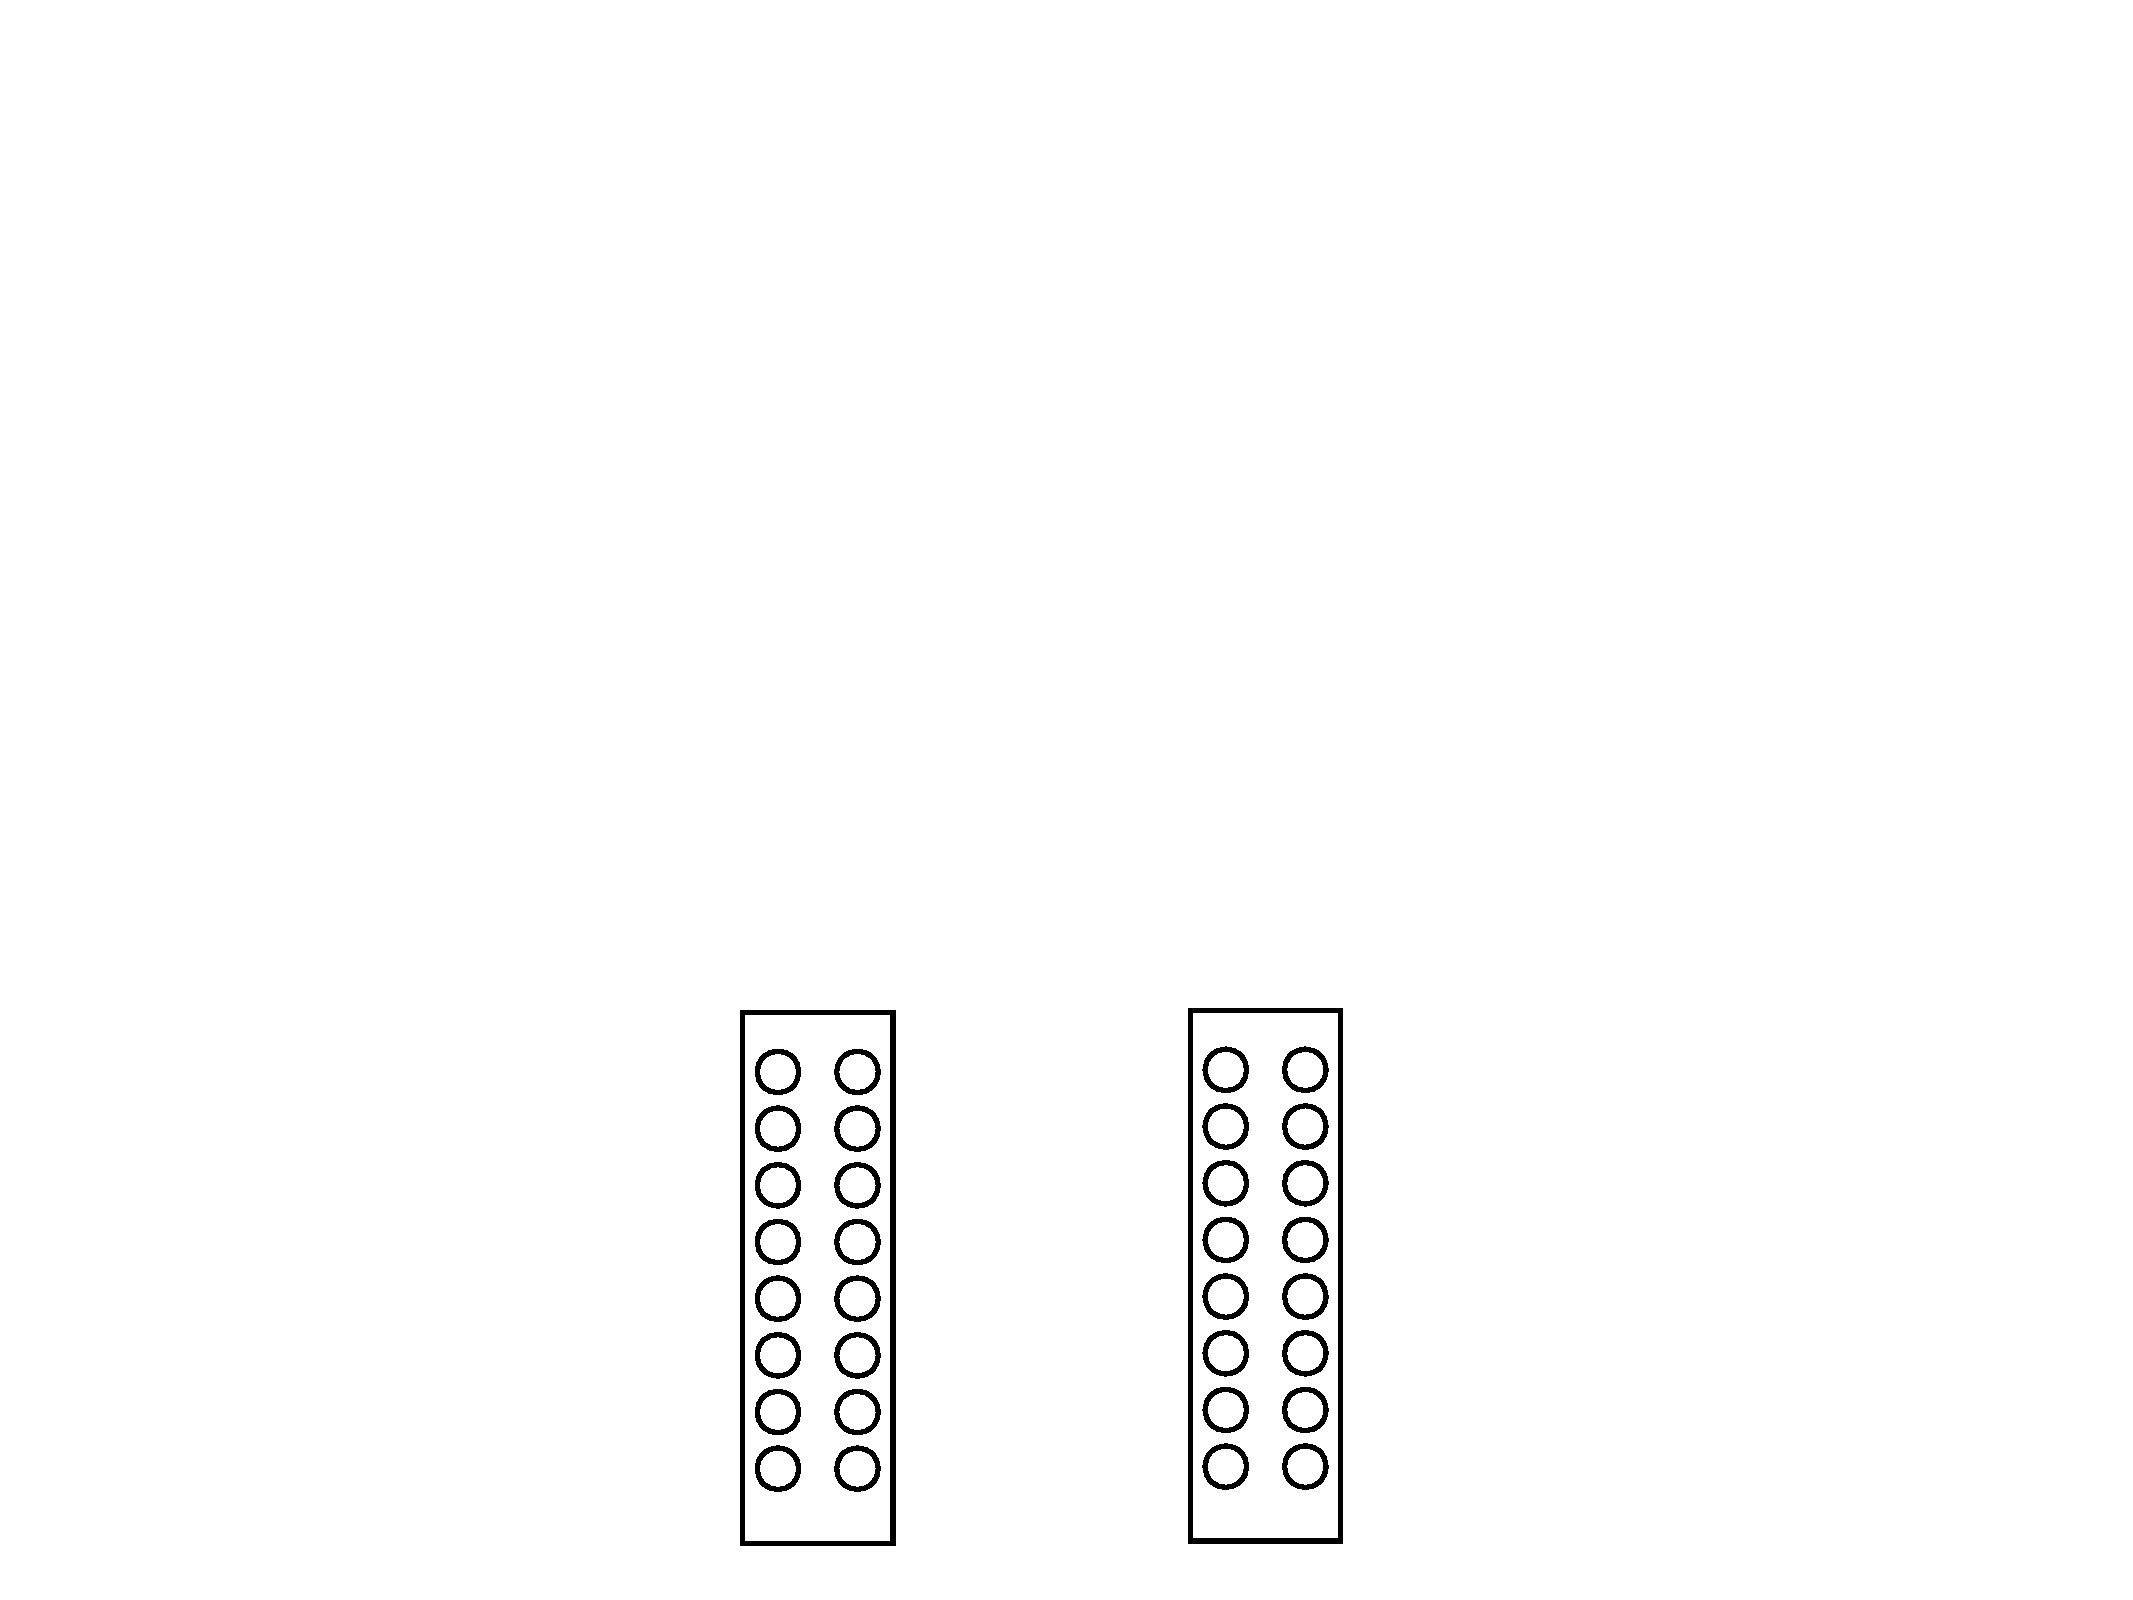
\includegraphics[width=.2\textwidth]{fig/plandetable.pdf}
    \end{center}
    \begin{definition}
        Un graphe non orienté est \emph{biparti} si l'ensemble des sommets peut être séparé en deux ensembles disjoints $S_1$ et $S_2$ tel que chaque arête du graphe relie un sommet de $S_1$ à un sommet de $S_2$ 
    \end{definition}
\end{frame}

\begin{frame}{Exemple}
    \begin{center}
    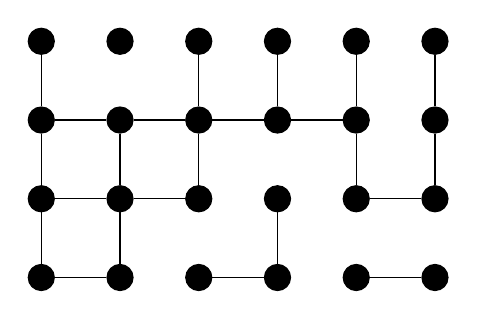
\begin{tikzpicture}
        \tikzstyle{sommet}=[circle,draw,fill=black]
        \node[sommet] (1) at (1,0) {};
        \node[sommet] (2) at (1,-1) {};
        \node[sommet] (3) at (1,-2) {};
        \node[sommet] (4) at (1,-3) {};
        \node[sommet] (5) at (2,0) {};
        \node[sommet] (6) at (2,-1) {};
        \node[sommet] (7) at (2,-2) {};
        \node[sommet] (8) at (2,-3) {};
        \node[sommet] (9) at (3,0) {};
        \node[sommet] (10) at (3,-1) {};
        \node[sommet] (11) at (3,-2) {};
        \node[sommet] (12) at (3,-3) {};
        \node[sommet] (13) at (4,0) {};
        \node[sommet] (14) at (4,-1) {};
        \node[sommet] (15) at (4,-2) {};
        \node[sommet] (16) at (4,-3) {};
        \node[sommet] (17) at (5,0) {};
        \node[sommet] (18) at (5,-1) {};
        \node[sommet] (19) at (5,-2) {};
        \node[sommet] (20) at (5,-3) {};
        \node[sommet] (21) at (6,0) {};
        \node[sommet] (22) at (6,-1) {};
        \node[sommet] (23) at (6,-2) {};
        \node[sommet] (24) at (6,-3) {};
        \draw (1) -- (2) -- (3) -- (4);
        \draw (6) -- (7) -- (8);
        \draw (9) -- (10) -- (11);
        \draw (13) -- (14);
        \draw (15) -- (16);
        \draw (17) -- (18) -- (19);
        \draw (21) -- (22) -- (23);
        \draw (2) -- (6) -- (10) -- (14) -- (18);
        \draw (3) -- (7) -- (11);
        \draw (19) -- (23);
        \draw (4) -- (8);
        \draw (12) -- (16);
        \draw (20) -- (24); 
    \end{tikzpicture}
\end{center}
\end{frame}

\begin{frame}{Exemple}
    \begin{center}
    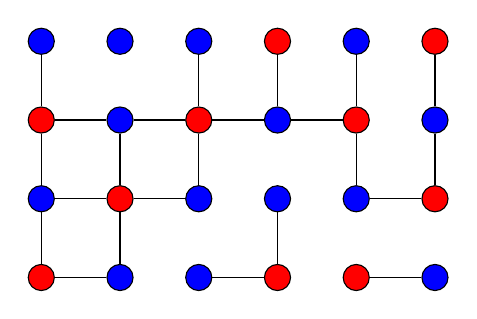
\begin{tikzpicture}
    \tikzstyle{sommetA}=[circle,draw,fill=blue]
    \tikzstyle{sommetB}=[circle,draw,fill=red]
    \node[sommetA] (1) at (1,0) {};
    \node[sommetB] (2) at (1,-1) {};
    \node[sommetA] (3) at (1,-2) {};
    \node[sommetB] (4) at (1,-3) {};
    \node[sommetA] (5) at (2,0) {};
    \node[sommetA] (6) at (2,-1) {};
    \node[sommetB] (7) at (2,-2) {};
    \node[sommetA] (8) at (2,-3) {};
    \node[sommetA] (9) at (3,0) {};
    \node[sommetB] (10) at (3,-1) {};
    \node[sommetA] (11) at (3,-2) {};
    \node[sommetA] (12) at (3,-3) {};
    \node[sommetB] (13) at (4,0) {};
    \node[sommetA] (14) at (4,-1) {};
    \node[sommetA] (15) at (4,-2) {};
    \node[sommetB] (16) at (4,-3) {};
    \node[sommetA] (17) at (5,0) {};
    \node[sommetB] (18) at (5,-1) {};
    \node[sommetA] (19) at (5,-2) {};
    \node[sommetB] (20) at (5,-3) {};
    \node[sommetB] (21) at (6,0) {};
    \node[sommetA] (22) at (6,-1) {};
    \node[sommetB] (23) at (6,-2) {};
    \node[sommetA] (24) at (6,-3) {};
    \draw (1) -- (2) -- (3) -- (4);
    \draw (6) -- (7) -- (8);
    \draw (9) -- (10) -- (11);
    \draw (13) -- (14);
    \draw (15) -- (16);
    \draw (17) -- (18) -- (19);
    \draw (21) -- (22) -- (23);
    \draw (2) -- (6) -- (10) -- (14) -- (18);
    \draw (3) -- (7) -- (11);
    \draw (19) -- (23);
    \draw (4) -- (8);
    \draw (12) -- (16);
    \draw (20) -- (24); 
\end{tikzpicture}
\end{center}
\end{frame}

\begin{frame}[fragile]
\frametitle{Algorithme : principe}

\begin{itemize}
    \item Pendant un parcours en profondeur, on associe une couleur (0 ou 1) à chaque sommet en s'assurant que deux sommets adjacents n'ont pas la même couleur 
    \item Si l'algorithme termine sans erreur, on a examiné chaque arête et attribué des couleurs cohérentes à chaque sommet : le graphe est biparti 
    \item Sinon, le coloriage est impossible et l'algorithme s'arrête avant la fin 
\end{itemize}
\end{frame}

    \begin{frame}[fragile]
        \frametitle{Algorithme}
            \begin{columns}
                \begin{column}{.55\textwidth}
                    \begin{algorithmic}
                    \Function{visite}{$i$ : sommet,$c$ : int}
                    \State vu[i] \gets true
                    \State couleur[i] \gets $c$
                    \For{$j \in Adj[i]$}
                        \If{$vu[j] = false$}
                            \State visite(j,1-$c$)
                        \ElsIf{couleur[j] = $c$} 
                                \State STOP("pas biparti")
                        \EndIf
                    \EndFor
                    \EndFunction
                                    \end{algorithmic}
                \end{column}
                \begin{column}{.45\textwidth}
                    \begin{algorithmic}
                        \State vu \gets [$false$,...,$false$]
                        \State couleur \gets $[-1,...,-1]$
                        \For{$i \in S$}
                            \If{$vu[i] = false$}
                                \State visite(i)
                            \EndIf
                        \EndFor
                    \end{algorithmic}            
                \end{column}
            \end{columns}    
        \end{frame}
        
\begin{frame}{k-coloration}
\begin{definition}
    Un graphe non-orienté est \emph{$k$-coloriable} si on peut colorier chaque sommet avec une couleur comprise entre $1$ et $k$, de telle façon que deux sommets adjacents aient des couleurs distinctes
\end{definition}
\begin{itemize}
    \item Remarques 
    \begin{itemize}
        \item Un graphe biparti est un graphe $2$-coloriable 
        \item L'algorithme de $2$-coloration vu précédemment est linéaire, ce n'est pas généralisable malheureusement
        \item De fait, pour $k>2$, le problème de déterminer si un graphe est $k$-coloriable est NP-complet  
    \end{itemize}
\end{itemize}
\end{frame}

% parcours en profondeur (version non récursive) 

\begin{frame}{Dérécursification}

\begin{itemize}
    \item Tout programme récursif peut être transformé en un programme équivalent non récursif, en s'aidant d'une \emph{pile} 
    \begin{itemize}
        \item cela peut avoir un intérêt pour l'efficacité (peu probable)
        \item certains compilateurs savent le faire automatiquement (HS ici) 
        \item dans certains cas, c'est plus facile à comprendre 
    \end{itemize}
\end{itemize}
\end{frame}

\begin{frame}[fragile]
    \frametitle{Algorithme de parcours en profondeur itératif}
        \begin{columns}
            \begin{column}{.55\textwidth}
                \begin{algorithmic}
                    \Function{visite}{$i$ : sommet}
                    \State P \gets empty() 
                    \State vi[i] \ gets true 
                    \State push(P,i) 
                    \While{!empty(P)}
                        \State k \gets pop(P)
                        \For{$j \in Adj[k]$}
                            \If{!vu[j]} 
                            \State vu[k] \gets true 
                            \State push(P,j
                            \EndIf
                        \EndFor
                    \EndWhile
                    \EndFunction
                \end{algorithmic}
            \end{column}
            \begin{column}{.45\textwidth}
                \begin{algorithmic}
                    \State vu \gets [$false$,...,$false$]
                    \For{$i \in S$}
                        \If{$vu[i] = false$}
                            \State visite(i)
                        \EndIf
                    \EndFor
                \end{algorithmic}            
            \end{column}
        \end{columns}    
    \end{frame}

